\documentclass[border=6pt]{standalone}
\usepackage{amsmath}
\usepackage{tikz}
\usetikzlibrary{arrows.meta}
\begin{document}
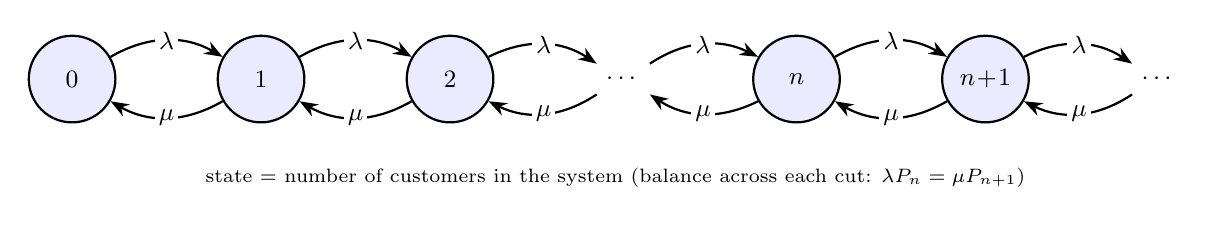
\begin{tikzpicture}[>=Stealth,font=\small,
 s/.style={draw,thick,circle,minimum size=1.1cm,inner sep=0pt,fill=blue!8},
 e/.style={->,thick},
 lab/.style={font=\small,fill=white,inner sep=1.5pt},
 every loop/.style={->,thick,looseness=6}]
\node[s] (0) at (0,0) {$0$};
\node[s] (1) at (2.4,0) {$1$};
\node[s] (2) at (4.8,0) {$2$};
\node (d) at (7.0,0) {$\cdots$};
\node[s] (n) at (9.2,0) {$n$};
\node[s] (n1) at (11.6,0) {$n\!+\!1$};
\node (d2) at (13.8,0) {$\cdots$};
\foreach \a/\b in {0/1,1/2,2/d,d/n,n/n1,n1/d2} {
  \draw[e] (\a) to[bend left=30] node[lab]{$\lambda$} (\b);
  \draw[e] (\b) to[bend left=30] node[lab]{$\mu$} (\a);
}
\node[font=\scriptsize] at (6.9,-1.25) {state = number of customers in the system (balance across each cut: $\lambda P_n=\mu P_{n+1}$)};
\end{tikzpicture}
\end{document}
